\documentclass[a4paper,16pt,UTF8]{article}
    % 宏包的使用
    \usepackage{ctex}
    \usepackage{titlesec} 
    \usepackage{graphicx}
    % \usepackage{float}
    \usepackage{geometry}
    \usepackage{multirow}
    \usepackage{booktabs}
    \usepackage{amsmath}
    \usepackage{amssymb}
    \usepackage{amsthm}
    \usepackage{mathrsfs}
    \usepackage{listings}
    \usepackage{abstract}
    \usepackage{color}
    % \usepackage{tabularx}
    \usepackage[fntef]{ctexcap}
    \usepackage{siunitx}
    \usepackage{enumerate}
    \usepackage{mdwlist}
    \usepackage{caption}


    % \newtheorem{theorem}{\hspace{2em}定理}[section]
    % \newtheorem{Definition}{\hspace{2em}定义}[section]
    % \newcommand{\ud}{\,\mathrm{d}}
    \graphicspath{{pic/}}

\begin{document}
    
\title{\Huge 图像理解 课程感想}
\author{指导教师 \quad 张绍明\\
        1551127 \quad 任家平}
\date{}
\maketitle

\section{\LARGE 图像的频率域}

\subsection{\large 傅里叶变换}
该文章转载于知乎

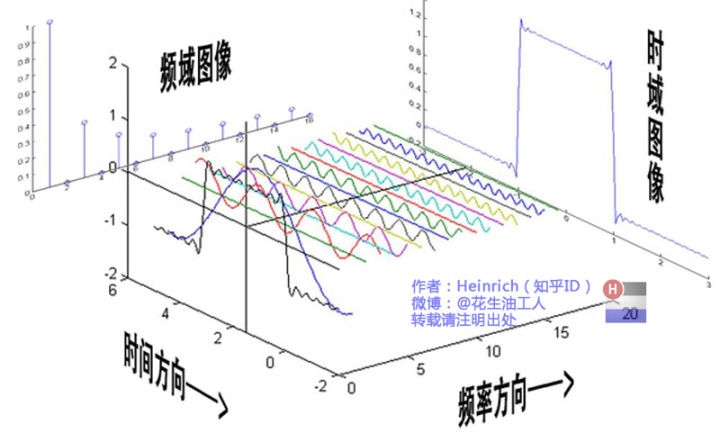
\includegraphics[width = 0.9\textwidth]{1.jpg}

如上图,将时间域中的一个矩形通过傅里叶变换转化为多个离散三角函数的叠加

下图则是将时间域中的一个矩形通过傅里叶变换转化为连续的三角函数叠加。

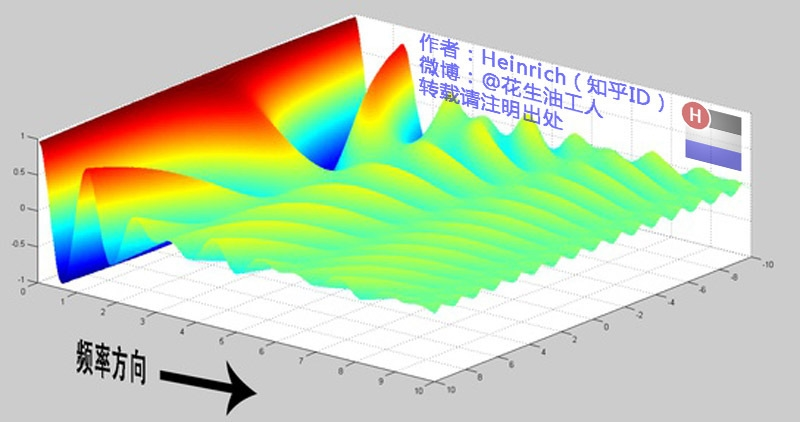
\includegraphics[width = 0.9\textwidth]{3.jpg}

如下图所示,在复数频率域通过傅里叶变换表示一个矩形波

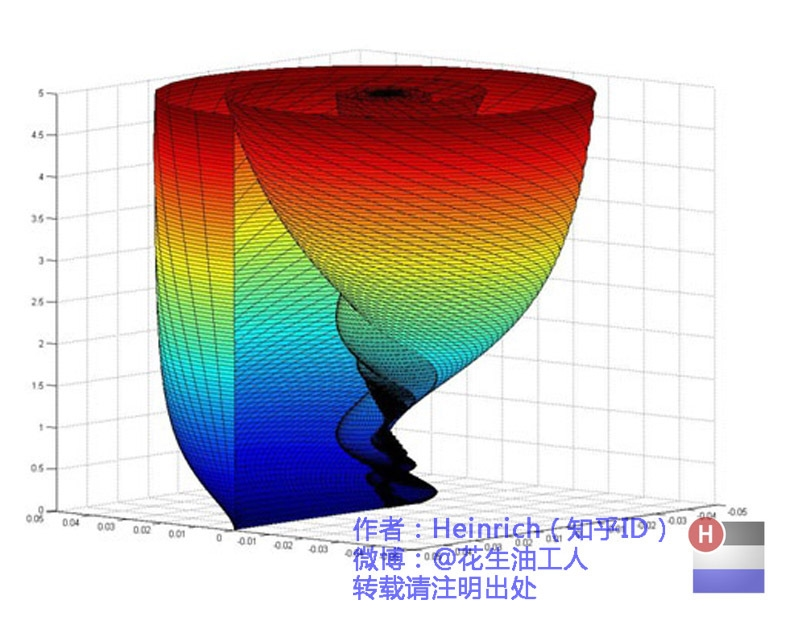
\includegraphics[width = 0.9\textwidth]{4.jpg}

由此,通过傅里叶变换,可将在时间域的一个矩形波在频率域和复数频率域有如下表示

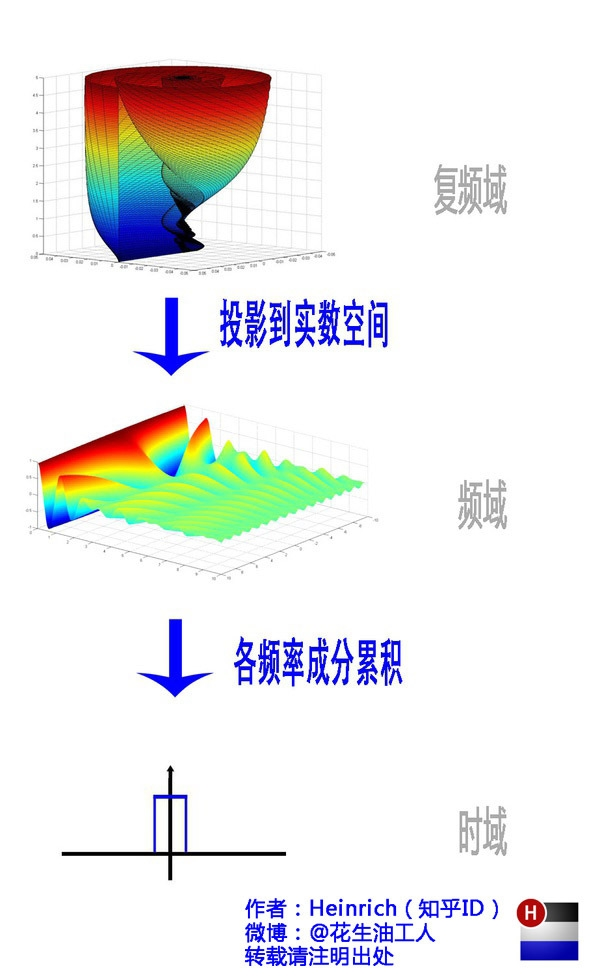
\includegraphics[width = 0.9\textwidth]{6.jpg}

由于在计算机中图像是离散信号,所以需要对传统的傅里叶变换进行改进,得出l冲击傅里叶变换DFT

\subsection{\large 图像的频率域}

上一部分理解了傅里叶变换和频率域,但是其针对的是时间域,对于图像的空间域的傅里叶变换,其频率域的定义又是如何?

$Fourier$变换便是
任何信号(包括图像信号)都可以表示成一系列正弦信号的叠加,在图像领域就是将图像灰度值作为正弦变量。可在单傅里叶中由三个分量编码:频率$f$、幅值$A$、相位$\varphi$,这三个值可以描述正弦图像中的所有信息。傅里叶变换同时将图像中所有频率进行编码:一个只包含一个频率f1的信号在频谱上横坐标f为f1的点处绘制一个单峰值,峰值高度等于对应的振幅,或者正弦曲线信号的高度。如下图所示。通常我们经常把傅里叶变换用对称的镜像表示,在原点的的两端,频率都是增加的方向,具有相同的幅值。如下图所示:

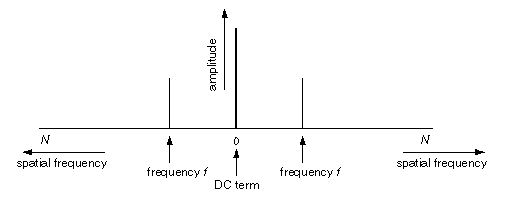
\includegraphics[width = 0.9\textwidth]{dft01.jpg}

上面讲的都是一维信号,一个二维傅里叶变换是一维傅里叶变换在每一个行扫描线和列扫描线上的傅里叶变换的叠加。其效果如下图所示:

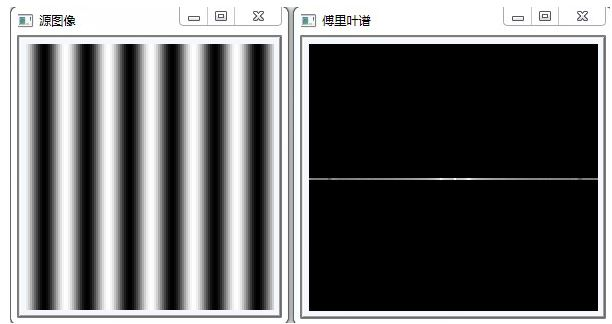
\includegraphics[width = 0.85\textwidth]{dft02.jpg}

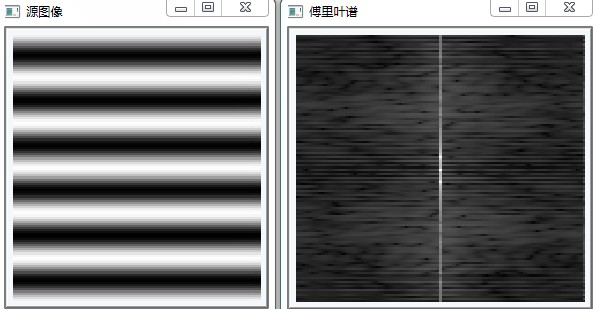
\includegraphics[width = 0.9\textwidth]{dft03.jpg}

\section{\LARGE 特征}

图像的特征:使计算机能够理解的“语言”描述图像中的标志性元素。为目标识别提供基础。

\subsection{\Large 点特征的提取与描述}

\begin{flushleft}
    \begin{description}
        \item[Harris算子]

        原理来源于人对角点的感性判断,即图像在各个方向灰度有明显变化。算法的核心是利用局部窗口在图像上进行移动判断灰度发生较大的变化来判断角点。

        Harris算子不具有尺度的描述能力

        \begin{equation*}
            E(u,v) = \sum_{x,y}w(x,y)\left[I(x+u,y+v) - I(x,y) \right]^{2}
        \end{equation*}

        对$E(u,v)$进行二次型的转换

        \begin{equation*}
            E(u,v) = 
            {\left[
                \begin{array}{c c}
                    u & v
                \end{array}
            \right]}
            \dot 
            {\left[
                \begin{array}{c c}
                    I_{x}^{2} & I_{x}I_{y} \\
                    I_{x}I_{y} & I_{y}^{2}
                \end{array}
             \right]}
            \dot
            {\left[
                \begin{array}{c}
                    u \\
                    v
                \end{array}
            \right]}
        \end{equation*}
        
        \begin{equation*}
            E(u,v) = 
            {\left[
                \begin{array}{c c}
                    u & v
                \end{array}
            \right]}
            \dot 
            M
            \dot
            {\left[
                \begin{array}{c}
                    u \\
                    v
                \end{array}
            \right]}
        \end{equation*}

        对$M$的特征值$\lambda1$,$\lambda2$进行分析,与平差中的误差椭圆类似,$\lambda1$,$\lambda2$表示的是在移动选择框时,灰度变化明显的两个方向。根据$\lambda1$,$\lambda2$两个大小关系可以判断出,点的属性。

        \item[高斯拉普拉斯算子LOG]

            具有尺度描述的能力,构建了英雄的的尺度空间金字塔,在尺度图像中,检测图像的二阶导,二阶导数的极大值可以突出角点

        \item[SIFT]

            全称$Scale-Invariant Feature Transform$
            相比前两个算子,SIFT算子还加上了旋转的方向信息。其步骤如下:
            \begin{enumerate}
                \item 搜索相邻尺度空间中的局部极大值点(DOG局部极大点)
                \item 去掉DOG值不够强的点和边缘点
                \item 计算每个兴趣点的HOG(Histogram of Gradient),并构成主方向对兴趣点进行描述
            \end{enumerate}

            之所以SIFT具有旋转尺度是由于神来之笔的主方向的定义。通过128维的方向向量找到了旋转尺度之间的关联。

            实验
            \begin{enumerate}
                \item 寻找特征点

                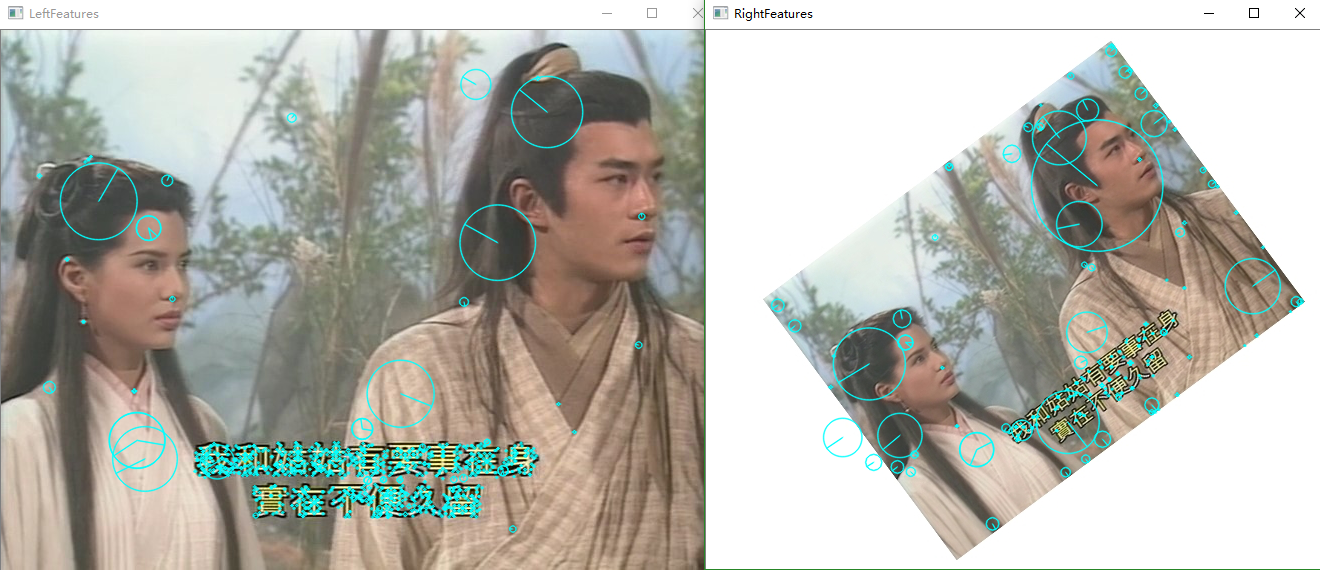
\includegraphics[width = 0.7\textwidth]{sift01.jpg}

                \item 根据主方向匹配并优化结果

                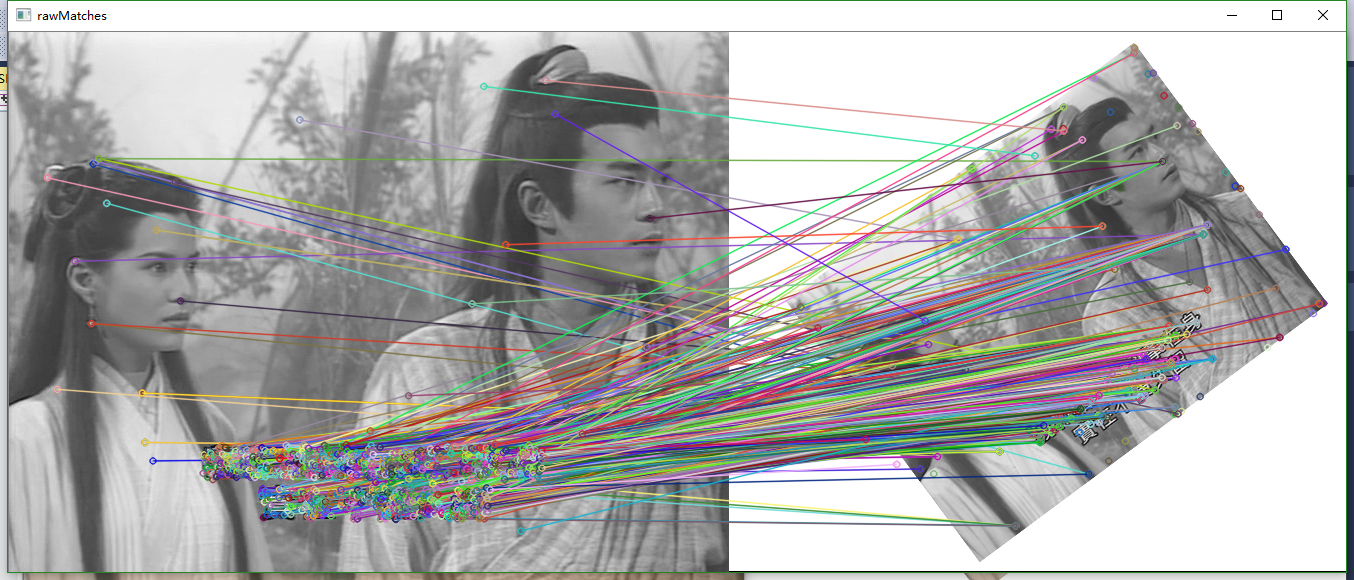
\includegraphics[width = 0.7\textwidth]{sift02.jpg}

                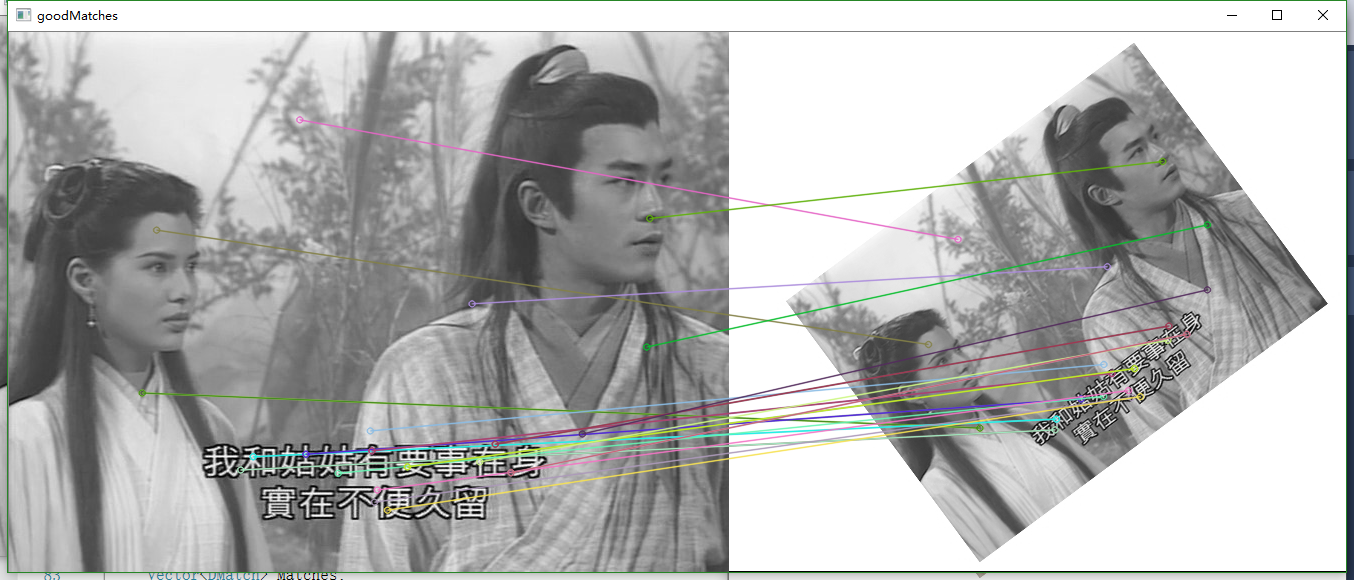
\includegraphics[width = 0.85\textwidth]{sift03.jpg}
                
                \item 计算变换矩阵并绘制矩形
                
                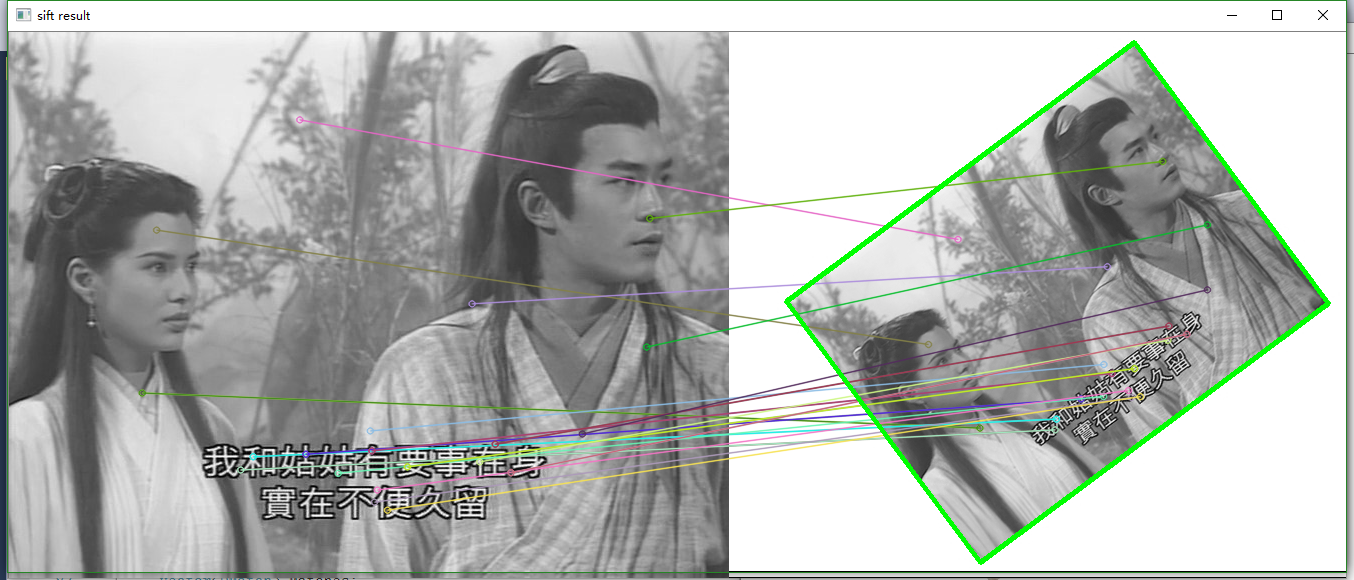
\includegraphics[width = 0.85\textwidth]{sift04.jpg}
            
            \end{enumerate}
            
    \end{description}
\end{flushleft}


\subsection{\Large 线特征的提取与描述}

\begin{description}
    \item[高斯拉普拉斯算子LOG]
    与点特征提取中不同,它所寻求的是二阶导的过零点
    \item[Canny算子]
    在梯度方向计算梯度模值的局部极大值

    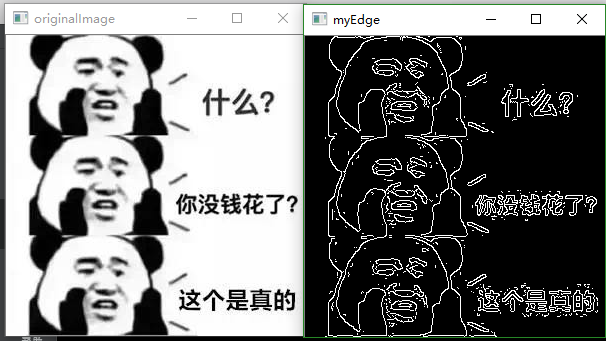
\includegraphics[width = 0.7\textwidth]{canny.jpg}

    \item[Hough变换]
    将曲线控件变换到参数空间,通过检测参数空间中的极值点,确定了描述该曲线的参数,从而提取了影像中的参数。

    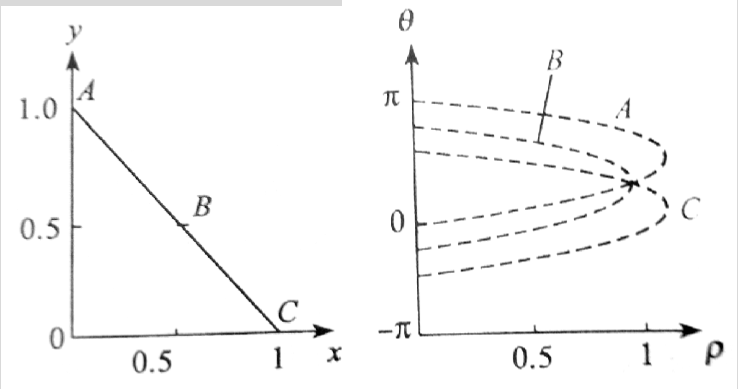
\includegraphics[width = 0.8\textwidth]{hough.jpg}

    一般在Hhough变换之前进行边缘检测。通常的用法是先用canny算子进行边缘检测,进行膨胀服饰等形态学的细化,然后再使用hough变化求解某些直线的参数,将求出的边缘参数化,用于计算。

    \item[LSD方法]

    全称$Line Segement Detector$,使用区域生长的方法,对已经处理过的像素标记进行标记,标记过的像素不再处理,在生长过程中,一要保证灰度的不变性,不能有显著差异.

    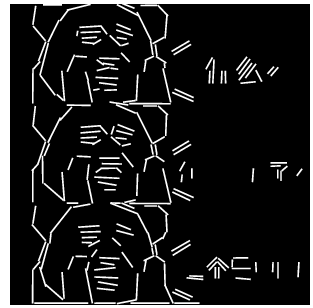
\includegraphics[width = 0.6\textwidth]{lsd.jpg}

\end{description}

\subsection{\Large 面特征的提取与描述}

一般用于描述图像的纹理特征的面特征识别方法
\begin{description}
    \item[灰度共生矩阵]
    对于任意平移量$(a,b)$,图像灰度阶数为$k$,则灰度共生矩阵的大小为$k^{2}$
    为了减少储存灰度共生矩阵所需要空间,一般先将图像降阶处理,然后再统计其灰度共生矩阵。

    \item[Gabor滤波器]

    Gabor滤波器的频率和方向表达同人类视觉系统类似,仿生的数学模型,十分适合纹理表达和分离。在空间域中,一个二维Gabor滤波器是一个由正弦平面波调制的高斯核函数。

    实在看不懂,只能会用

    \item[HOG]
    在SIFT中使用,对图像通过设置block和cell来完成面特征的提取

\end{description}

多用于图像的分类的面特征识别
\begin{description}
    \item[OSTU阈值分割]
    主要用于前景和背景的分类, 对于一幅图像,设当前景与背景的分割阈值为t时,前景点占图像比例为$w0$,均值为$u0$,背景点占图像比例为$w1$,均值为$u1$。则整个图像的均值为$u = w0*u0+w1*u1$。建立目标函数$g(t)=w0*(u0-u)^2+w1*(u1-u)^2$,$g(t)$就是当分割阈值为t时的类间方差表达式。OTSU算法使得g(t)取得全局最大值,当g(t)为最大时所对应的t称为最佳阈值。OTSU算法又称为最大类间方差法。
    \item[极大似然方法]
    统计图像灰度直方图,根据波谷得出不同地物的阈值,之后分类,其数学原理为贝叶斯定律。
    \item[区域生长与标记]
    和面特征的LSD有相似性,只不过这时生长的标准不再是梯度值而是像素值。
    \item[K均值聚类法]
    需要在分类之前知道类别的个数k,设置质心,计算各个簇的SSE作为评判的参数,通过迭代直到质心满足条件或是达到最大迭代次数。

\end{description}

\section{\LARGE 机器学习初识}

这一部分也只能听个大懂,考完试慢慢看。
现在理出来的思路为:

\begin{enumerate}
    \item 二值分类引出感知机(损失函数,梯度下降)
    \item 多值分类引出计算机对亦或的学习能力
    \item 为了解决Xor能力,提出两个解决方案,靠深度解决维度问题(人工神经网络),靠核函数解决维度问题(支持向量积)
\end{enumerate}

感知机是一个信号的转换,对A类将其标识为1,对B类将其标识为-1或者0
\begin{equation*}
    g(x) = \left \{ 
        \begin{array}{c c c c}
            A &=&1 & {f(x) \leq 0}\\
            B &=&-1 & {f(x) \geq 0}
        \end{array} 
        \right.
\end{equation*}

神经网络大致结构是输入层,隐含层和输出层。先需要样本的训练,得出隐含层中的参数,所以能否分类正确和样本的选择息息相关。之前在SITP项目中用过BP神经网络,当时连BP代表什么都不知道,只是为了解决问题(增加逼格),硬往上套,只是大略明白了神经网络的原理,但是具体如何调整参数,不同的神经网络其调整方法不同。BP是回溯,从结果往前推出每个合适的参数。还有径向基网络、自由竞争网络、循环网络等等

支持向量积的主要思想可以概括为两点
\begin{enumerate}
    \item 它是针对线性可分情况进行分析,对于线性不可分的情况,通过使用非线性映射算法将低维输入空间线性不可分的样本转化为高维特征空间使其线性可分,从而使得高维特征空间采用线性算法对样本的非线性特征进行分析成为可能。
    \item SVM方法是通过一个非线性映射p,把样本空间映射到一个高维乃至无穷维的特征空间中(Hilbert空间),使得在原来的样本空间中非线性可分的问题转化为在特征空间中的线性可分问题。简单地说,就是升维和线性化。升维,就是把样本向高维空间做映射,一般情况下这会增加计算的复杂性,甚至会引起“维数灾难”,
\end{enumerate}
其核函数将特征进行从低维到高维的转换,但核函数事先在低维上进行计算,而将实质上的分类效果表现在了高维上,避免了直接在高维空间中的复杂计算。

\section{实验}

一开始是想通过分析图像的直方图,自己从底层搞出一套非监督分类方法,但是发现按照老师的路子走,LAB空间分解,之后通过极大似然的分类法则,分出印章背景和文字。但是无论怎么分,都不能准确的分出印章,因为中间的背景部分会存在部分红色。一旦光照条件发生变化,就算是提前做过了均衡化,也会存在较多的误分情况。

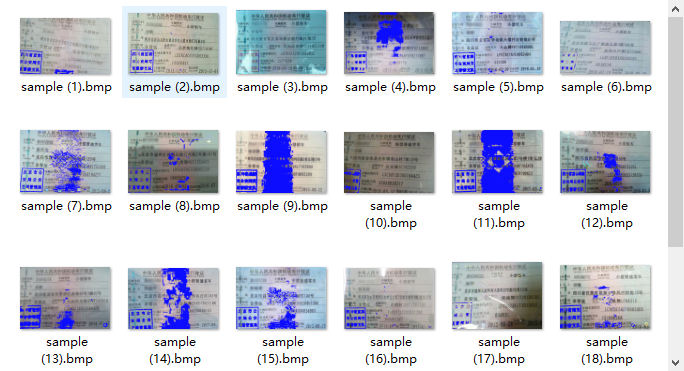
\includegraphics[width = 0.7\textwidth]{test01.jpg}

之后觉得可以限定印章的xy范围,但是限定之后,那么监督分类方法失去了意义,它变成了苦力活。所以改用OSTU大津阈值分割法进行,好处是最大类间内方差,无需担心光照的变化,但是分割出来的印章过粗。忽略这一点之后用opencv自带的阈值分割是可以做到印章背景文字三者的分类。

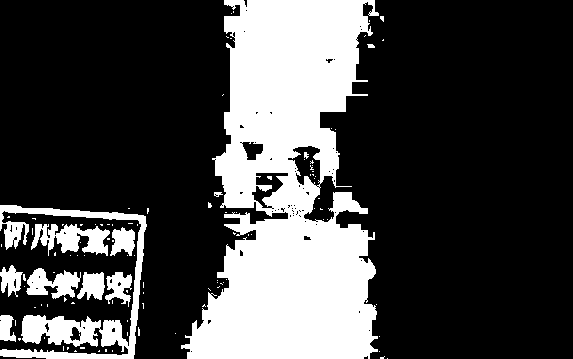
\includegraphics[width = 0.8\textwidth]{test03.jpg}

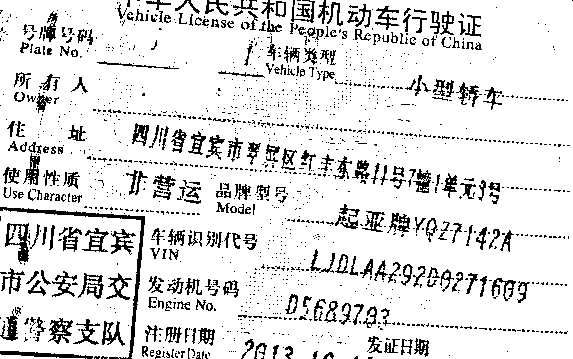
\includegraphics[width = 0.8\textwidth]{test02.jpg}

看了大家做的实验项目,我觉得章学城同学做的很优秀。首先他没有使用任何的深度学习或是人工智能的方法,完全使用非监督分类,先是限定范围的OSTU,之后gabor滤波器,阈值分割,然后膨胀腐蚀,得出最终的文字块和印章。我觉得分的很完美。

\section{感想}

相对于学院的其他课程,图像分析与理解(数字图像处理2)这门课比较系统、专业更重要的是贴近现实。传统测量讲的极为系统专业,但以后的路子感觉只有令人难过的高校或是测绘局;吴杭彬老师的数据通讯编程课不够系统也不够专业,不过下午的计算机图形学倒是不错,就是cad附带vba二次开发的环境是80年代的古董,居然不会自动释放局部变量;杨光老师和刘世杰老师的编程课只是为了满足课程设计的要求,浅浅地讲了讲程序;王卫安老师的图像理解与分析很不错,是一门图像的基础课。所以还是老师您的课程可以让人在多方面感到满意。

图像理解的基础虽然不是很乐观,路很长,慢慢来。
\end{document}